\chapter{Grundlagen der Softwarearchitektur}
\label{chap:theo_softw_archit}
In diesem Kapitel werden Grundlagen der Softwarearchitektur im Hause \gls{arburg} aufgezeigt. 

\section{.NET}
\label{sec:dotnet}
Beim \gls{dotnet_framework}-Framework handelt es sich um eine Softwareplattform von Microsoft, welche die Anwendungsentwicklung für Microsoft-Betriebssysteme vereinheitlicht. Es eignet sich für Webseiten, Services und Desktop-Apps \cite{dotnetArchitecture}. Zum einen stellt es eine Klassenbibliothek für umfangreiche Funktionalitäten zur Verfügung. Zum anderen wird mit der \gls{clr} eine Laufzeitumgebung bereitgestellt, welche sich unter anderem um die Ausführung von Anwendungen, Garbage Collection und Thread-Management kümmert. Die Applikationen können in C-Sharp, F-Sharp oder Visual Basic geschrieben werden. Sie werden in einen sprachunabhängigen \textit{Intermediate Language Code} kompiliert und in Assemblys gespeichert (.dll/.exe). Bei der Ausführung einer Applikation übersetzt ein just-in-time Compiler diese Assemblys in Maschinencode, der auf dem jeweiligen Computer ausgeführt werden kann \cite{dotnetArchitecture}. 

Für ein besseres Verständnis später folgender Code-Ausschnitte folgt eine Erklärung zu zwei Funktionalitäten in \gls{dotnet_framework}.

Out-Parameter werden durch das Schlüsselwort \textit{out} festgelegt. Sie ermöglichen eine Rückgabe des Erfolges als auch des gesuchten Wertes. Somit wird direkt überprüft, ob weiter mit diesem Wert gearbeitet werden kann. 

\begin{lstlisting}[caption=Beispiel zu out-Parametern, label=lst:exa_out]
	private bool TryGetValue(out int value)
	{
		value = valueService.GetValue();
		if(value == null) return false;
		else return true;
	}
\end{lstlisting}

Optionale Parameter werden durch den Zusatz \textit{= null} festgelegt. Beim Aufruf kann ein optionaler Parameter entweder gesetzt werden oder nicht. Auch eine Variable mit dem Wert \textit{null} kann übergeben werden. Ersetzbar wäre diese Methode durch Überladung. In der Implementierung ist diese Lösung jedoch notwendig aufgrund von Polymorphie (\autoref{label:polymorph}). 

\begin{lstlisting}[caption=Beispiel zu optionalen Parametern, label=lst:exa_opt]
	private void ExecuteCommand(string name = null)
	{
		if(name != null) [...]
		else [...]
	}
\end{lstlisting}

\section{Objektorientierung}
\label{sec:oop}
\gls{oop} ist ein Konzept zur Minderung von Komplexität in der Softwareentwicklung. Es werden Klassen und Objekte genutzt, um eine Software zu strukturieren. Die Grundelemente der \gls{oop} sind:
\begin{itemize}
	\item Datenkapselung: Daten gehören explizit zu einem Objekt, ein Zugriff kann nur für Berechtigte über eine klar definierte Schnittstelle erfolgen (Beispielweise über \gls{getter}). Die Konsistenz der Daten kann somit besser sichergestellt werden \cite{LahresRayman}. Programmteile haben nur auf das Zugriff, dass sie benötigen. 
	\item \label{label:polymorph} Polymorphie: Eine Oberklasse gibt die Grundstruktur an, erbende Klassen implementieren diese in verschiedenen Ausführungen. Beispielsweise hat der Obertyp \textit{Tier} die Methoden \textit{fortbewegen} und \textit{ernähren}. Davon erben die Untertypen \textit{Haifisch} und \textit{Kamel}. Beide bewegen sich fort und ernähren sich. Der \textit{Haifisch} \textit{schwimmt} und \textit{jagt Tiere}. Das Kamel dagegen \textit{läuft} und \textit{frisst Pflanzen}. Die gleichnamigen Methoden werden also unterschiedlich implementiert. Nun kann im Programm abstrakt \textit{Tier} verwendet und die Methode \textit{ernähren} aufgerufen werden. Erst zur Laufzeit (auch spätes Binden genannt), je nach Zuweisung eines Objektes, wird entschieden, ob die Methode beim \textit{Haifisch} oder \textit{Kamel} ausgeführt wird. Dies sorgt für Austausch-, Änder- und Erweiterbarkeit \cite{LahresRayman}. 
	\item Vererbung: Attribute und Methoden einer Oberklasse können an Unterklassen weitergegeben und somit wiederverwendet werden. Das Beispiel aus der Polymorphie wird erneut aufgegriffen. Sowohl \textit{Haifisch} als auch \textit{Kamel} besitzen Attribute wie \textit{Größe}, \textit{Gewicht} und \textit{Schnelligkeit}. Im Falle der Vererbung können diese direkt von der Oberklasse übernommen werden. Dies verhindert Redundanz und fördert Wiederverwendbarkeit \cite{LahresRayman}. Auch redundante Methoden können von der Oberklasse genutzt werden. 
\end{itemize}

\section{Composite Components und Dependency Inversion}
\label{sec:compositecomponents}
Die \acrlong{cca} zielt auf eine Entkopplung von Abhängigkeiten auf Komponenten-Ebene. Im Fall von \gls{arburg} ist damit die Projektebene gemeint. Dependency Inversion verfolgt dieses Ziel auf Klassenebene. Konkret soll eine Abhängigkeit nur von Abstraktionen und nicht von Details stattfinden. 
Dies wird durch die Trennung einer Komponente in den Implementierungsteil und Contracts-Teil (zu Deutsch: Vertrag) erreicht. Für jede Implementierung einer Komponente gibt es auch einen Contract. Dieser besteht letztlich aus Schnittstellen und Datenklassen. Es findet also eine Abstrahierung statt. Abhängigkeiten dürfen dabei nur zu Contracts bestehen (siehe \autoref{fig:compcomp}) und nicht zu Implementierungen. Dies soll für eine bessere Änder- und Austauschbarkeit sorgen, denn der Contract bleibt bestehen, während die Implementierung angepasst oder ausgetauscht werden kann \cite{Tielke.2015b}. 

\begin{figure}[!htb] 
	\centering
	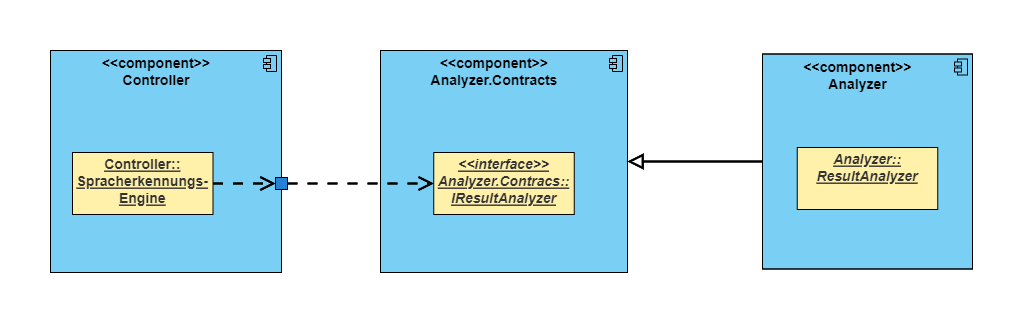
\includegraphics[width=16cm]{compcomp.png}
	\caption{Composite Components}
	\label{fig:compcomp}
\end{figure}
\FloatBarrier

\section{Dependency Injection}
\label{sec:dependencyinjection}
Ein Entwurfsmuster aus der Objektorientierung ist die \gls{di}, also Abhängigkeitsinjektion. Es soll Abhängigkeiten entkoppeln und auf ein Minimum reduzieren. Dabei handelt es sich um eine Weiterentwicklung der \textit{Inversion of Control} aus 2004 durch Martin Fowler \cite{Fowler.2004}. Konkret umgesetzt wird dies durch eine Fabrik oder einen Container, in welchen Objekte zentral erzeugt werden. Dieser injiziert diese dann passend, wenn benötigt. Folgend ein Beispiel:

\begin{figure}[!htb] 
	\centering
	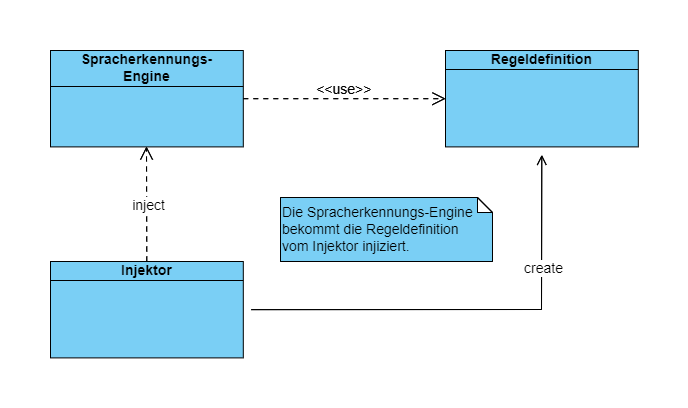
\includegraphics[width=12cm]{dependency_injection.png}
	\caption{Dependency Injection}
	\label{fig:dependency_injection}
\end{figure}
\FloatBarrier

Im Beispiel (siehe \autoref{fig:dependency_injection}) braucht die \textit{Spacherkennungsengine} eine Instanz der \textit{Regeldefinition}. Diese wird zentral im Injektor erzeugt und ihr dann injiziert. Dazu wird zwischen drei Methoden unterschieden \cite{Fowler.2004}, im Unternehmen \gls{arburg} wird folgende genutzt:
\begin{itemize}
	\item Constructor Injection: Die Abhängigkeit wird direkt im Konstruktor als Argument übergeben. 
\end{itemize}

Die Objekte müssen dabei einmalig dem \gls{di}-Container zugewiesen werden. Dies sieht folgendermaßen aus.

\begin{lstlisting}[caption=Dependency Injection, label=lst:depInj]
	this.ExportPart<ISpeechAssist, SpeechAssist>().AsSingleton();
	this.ExportPart<ITextResourcesExtractor, TextResourcesExtractor>();
	this.ExportPart<ITokenHolder, TokenHolder>().AsSingleton();
	this.ExportPart<IResultAnalyzer, ResultAnalyzer>();
\end{lstlisting}

Gemäß dem Dependency Inversion Prinzip (siehe \autoref{sec:compositecomponents}) wird jeder Implementierung eine Abstraktion zugeordnet. Die Instanzen können als einmalig, also als Singleton, definiert werden, um immer das gleiche Objekt zu nutzen. 